\label{subseq:mm-conclusion}

In this chapter, we have examined different types of sparse linear solvers applied to linear systems generated by ATHLET software resulting from thermo-hydraulic simulations. We have come to the conclusion that, in spite of better scalability and parallel efficiency of iterative methods, direct sparse linear solvers are most suitable for this purpose because of its robustness.\\


In subsection \ref{subseq:mm-library-choice}, we have tested different direct sparse solvers, namely: SuperLU\_DIST, PasTiX and MUMPS. MUMPS library showed better parallel performance among the others according to results of testing and, therefore, was chosen for the rest of the study where we focused on performance tuning of the library.\\


We have shown in subsequent subsections there have been four main sources of MUMPS library tuning, namely:

\begin{enumerate}
	\item correct selection of a fill reducing reordering method \label{conclusion:mm-1}
	\item destribution of MPI process among multiple NUMA domain within a compute node \label{conclusion:mm-2}
	\item configuration of MUMPS library with an optimal, tuned BLAS implementaion \label{conclusion:mm-3}
	\item execution of MUMPS with an optimal hybrid MPI/OpenMP mode \label{conclusion:mm-4}
\end{enumerate}


To perform accurate testing and careful analysis, two different matrix sets were used, namely: GRS and SuiteSparse. The fist one was a problem specific for thermo-hydraulic simulations whereas the second one was generated from SuiteSparse Matrix Collection \cite{sparse-matrix-collection:1}, \cite{sparse-matrix-collection:2} by downloading a dozen different matrices with respect to different number of equations and the number of non-zero elements. Additionally, some tests were performed on two different compute clusters, namely: HW1 and HW2 (see chapter \ref{subseq:matrix-sets-and-hardware}), to check whether results of testing were consistent between different hardware and operating environment or not.\\



\ref{conclusion:mm-1}. In subsection \ref{subseq:fill-in-reordering} it has been shown that parallel performance of MUMPS is quite sensitive to a used fill-in reducing reordering algorithm. A correct choice of an algorithm can lead to significant improvements in terms of the overall execution time. The average performance gain was almost \textbf{15\%} and in some particular cases it was possible to reduce execution time in approximately \textbf{40-55\%} in case of GRS matrix set. During experiments, we came to the conclusion there was no an indirect metric to predict the best algorithm in advance for a specific system of equations.\\


%%%%%%%%%%%%%%%%%%%%%%%%%%%%%%%%%%%%%%%%%%%%%%
\ref{conclusion:mm-2}. In section \ref{subseq:mm-mumps-process-pinning}, influence of different process pinning strategies on MUMPS parallel performance has been demonstrated. The tests have shown that equal distribution of MPI process among all available NUMA domains always bring extra performance. In average, \textit{spread}-pinning allows to reduce execution time of MUMPS by almost \textbf{5.5\%} and \textbf{13.8\%} on HW1 and HW2 machines, respectively, in case of GRS matrix set.\\


%%%%%%%%%%%%%%%%%%%%%%%%%%%%%%%%%%%%%%%%%%%%%%
\ref{conclusion:mm-3}. 
We have discussed and examined in section \ref{subseq:blas-comparison} the way how MUMPS library has been implemented to preform partial factorization of type 2 nodes in section. It has turned out the library intensively calls \textit{GEMM}, \textit{TRSM} and \textit{GETRF} BLAS subroutines. Therefore, replacement of standard Netlib BLAS library by tuned BLAS implementations makes it possible to improve overall performance of the solver in case of a sufficient amount of type 2 nodes in a matrix assembly tree.\\


The results have shown that OpenBLAS outperforms both Netlib and Intel MKL libraries, which were available for the tests, in case of GRS matrix set. The average performance gain turned out to be about \textbf{13\%} relatively to the default Netlib implementation and approximately \textbf{21\%} in contrast to Intel MKL library. We have also noticed that Intel MKL was even slower than Netlib BLAS for small and medium size GRS matrices in almost \textbf{52\%} and \textbf{2\%}, respectively. At the same time, both libraries, OpenBLAS and Intel MKL, showed significant performance gain relatively to the standard Netlib BLAS in case of SuiteSparse matrix set and allowed to reduce the execution time by almost \textbf{50\%} in average. \\


%%%%%%%%%%%%%%%%%%%%%%%%%%%%%%%%%%%%%%%%%%%%%%
%{subseq:mpi-openmp}
\ref{conclusion:mm-4}. In section \ref{subseq:mpi-openmp}, we have discussed where and how developers of MUMPS library applied shared-memory parallelism based on review of works \cite{chowdhury2010some} and \cite{l2013introduction}. \todo{problems with open blas} \todo{intel mkl}. We have also found severe slow-down of some hybrid MPI/OpenMP modes due to system and application thread conflicts  while MUMPS-OpenMP configuration was running on HW1 cluster. For that reason, the following study was continued with only using Intel MKL library which, in its turn, turned out to be thread-safe.\\


We have shown that in some particular cases, factorization of \textit{Geo\_1438} matrix for example, hybrid MPI-OpenMP approach can bring significant performance improvement. However, application of hybrid computing to GRS matrix set gives negligible improvement on HW1 machine i.e. around \textbf{2.1\%}, and significantly deteriorates parallel efficiency. Much optimistic results were obtained for experiments conducted on HW2 machine were performance gain reached almost \textbf{31\%} for the same matrix set. \\


During the study, we have also discovered the optimal hybrid MPI/OpenMP mode locates near the saturation point of the corresponding flat-MPI test. This fact can allow to reduce the amount of testing in general. However, we do not recommend to proceed the study in this direction due to above mention parallel efficiency issues detected on HW1 machine and lack of ability to run OpenBLAS library without thread conflicts.\\


Figures \ref{fig:mumps-final-comparison-1} and \ref{fig:mumps-final-comparison-2} show a comparison of MUMPS parallel performance before and after application of above mentioned tuning to GRS matrix set. In case of experiments labeled as \textit{default}, we used ParMetis as a fill reducing reordering algorithm because it had been used by GRS engineers before the current study.\\


\figpointer{\ref{fig:mumps-final-comparison-1}}
\begin{figure}[!htb]
\centering
	\begin{tabular}{cc}
		\subfloat[small system: cube-5]{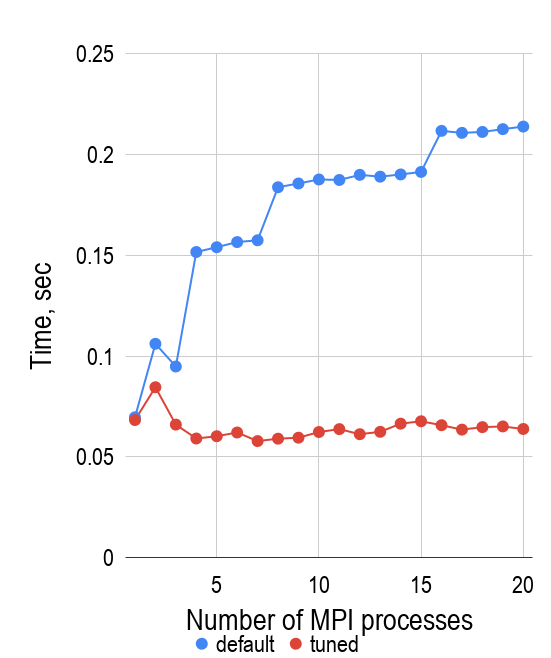
\includegraphics[width=0.43\textwidth]{figures/chapter-2/final-comparison/cube-5.png}} &
		\subfloat[small system: pwr-3d]{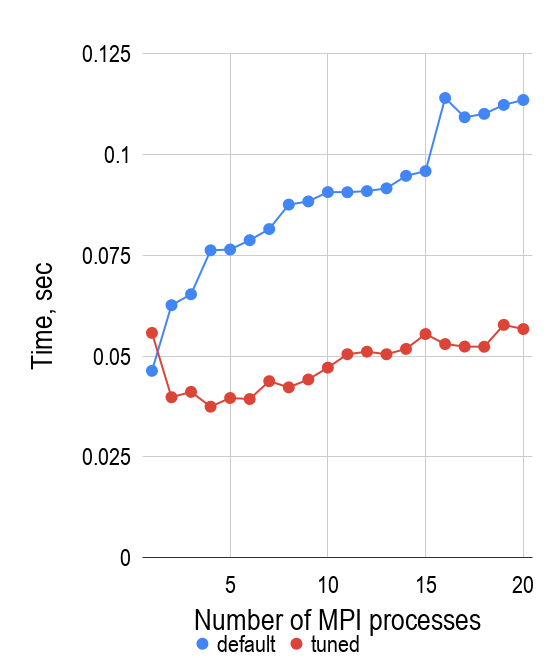
\includegraphics[width=0.43\textwidth]{figures/chapter-2/final-comparison/pwr-3d.png}} \\
	\end{tabular}
	\caption{MUMPS: comparison of different BLAS libraries with using both GRS and SuiteSparse matrix sets on HW1 machine}
	\label{fig:mumps-final-comparison-1}
\end{figure}



\figpointer{\ref{fig:mumps-final-comparison-2}}
\begin{figure}[!htb]
\centering
	\begin{tabular}{cc}
		\subfloat[medium system: cube-64]{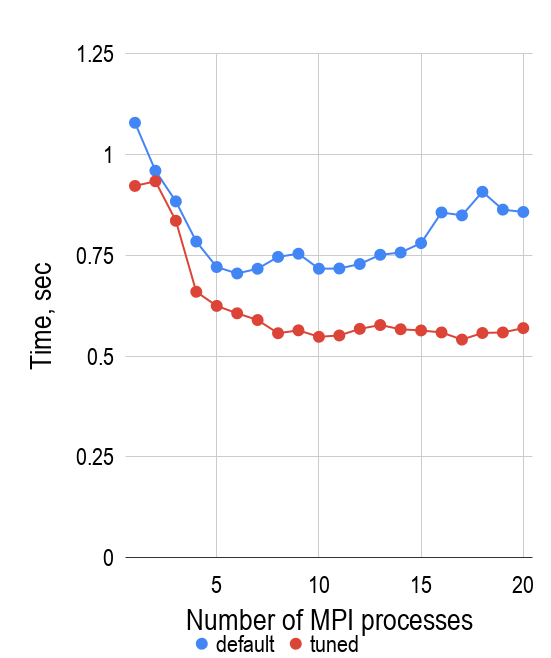
\includegraphics[width=0.48\textwidth]{figures/chapter-2/final-comparison/cube-64.png}} & 			        \subfloat[medium system: k3-2]{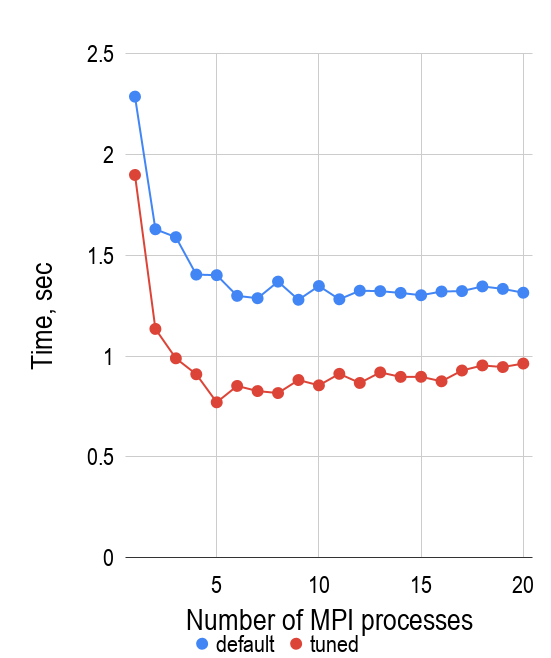
\includegraphics[width=0.48\textwidth]{figures/chapter-2/final-comparison/k3-2.png}} \\
		\subfloat[large system: cube-645\label{fig:mumps-final-comparison-cube-645}]{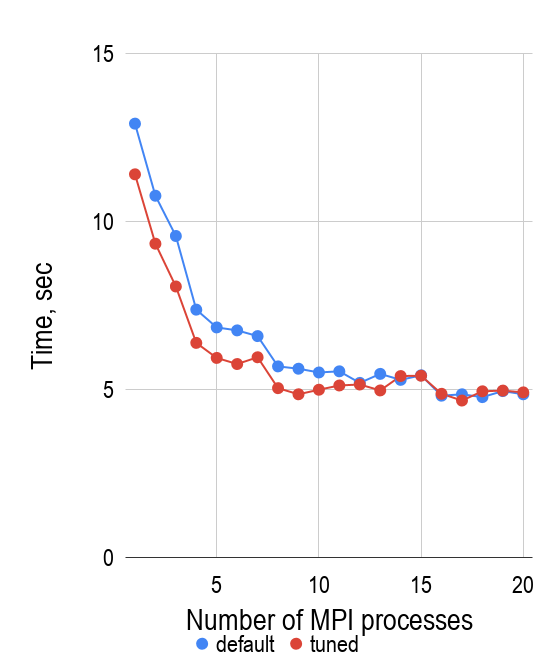
\includegraphics[width=0.48\textwidth]{figures/chapter-2/final-comparison/cube-645.png}} & 			        \subfloat[large system: k3-18\label{fig:mumps-final-comparison-k3-18}]{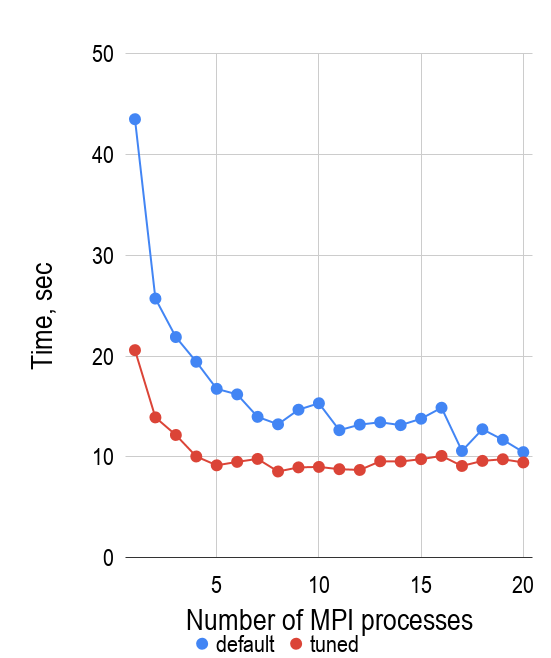
\includegraphics[width=0.48\textwidth]{figures/chapter-2/final-comparison/k3-18.png}} \\
	\end{tabular}
	\caption{MUMPS: comparison of different BLAS libraries with using both GRS and SuiteSparse matrix sets on HW1 machine}
	\label{fig:mumps-final-comparison-2}
\end{figure}



\todo{include statistics}
By and large, we have observed significant improvement of applied tuning techniques, mentioned above, for the entire GRS matrix set. \\


In average, the factorization time has been reduced in \textbf{51.4\%} for small sized systems. The significant performance gain mainly came from the optimal choice of fill-in reduction algorithm. Moreover, application of PT-Scotch for small sized systems allowed to drastically change strong scaling behavior and reduce the execution time by approximately \textbf{17\%} in contrast to sequential execution of the default MUMPS configuration that was a challenge before the study.\\


% medium sized systems
The execution time spent on factorization of medium sized systems dropped in \textbf{1.4} times. Additionally, we have noticed that scaling of \textit{cube-64} test case has been considerably changed as it happened in case of small sized systems. Application of PT-Scotch, to \textit{cube-64}, allowed to shift the saturation point from 5 to 10 process count without significant drop of parallel efficiency. All in all, tuning of MUMPS made it possible to reduce the execution time around the saturation points in almost \textbf{31\%} in average for medium sized GRS systems of equations.\\


% larged sized sized system
The factorization performance gain of large sized systems manly came from configuration of MUMPS with optimized BLAS library, OpenBLAS, and MPI \textit{spread} process distribution because it turned out that ParMetis was the best fill-in reduction algorithm for large systems. A noticeable performance gain difference was observed between \textit{cube-645} and \textit{k3-18} test cases. In average, run-time of MUMPS-OpenBLAS configuration reduced by almost \textbf{20\%} in contrast to the default installation in case of \textit{k3-18} whereas factorization time of \textit{cube-645} was improved only by 
\textbf{1.3\%}. However, the saturation points of both cases were shifted towards lower values of the process count which allows to considerably improve hardware utilization  together with improvement of library performance. For example, a detailed study of \textit{k3-18} performance graph, figure \ref{fig:mumps-final-comparison-k3-18}, shows that the saturation point has been moved from 17 to 8 process count. At the same time, the execution time drops by almost \textbf{19\%} and parallel efficiency jumped in about \textbf{13\%}. The same but less significant results can be observed for \textit{cube-645} test case, figure \ref{fig:mumps-final-comparison-cube-645}. \\



%average
% shit of saturation point
% usage of less amount of processing units helps to improve efficiency of the system
% example of k-18, k3-2
% recomendations for small, medium and big GRS systems

\newpage